\documentclass[14pt]{extbook}
\usepackage{multicol, enumerate, enumitem, hyperref, color, soul, setspace, parskip, fancyhdr} %General Packages
\usepackage{amssymb, amsthm, amsmath, bbm, latexsym, units, mathtools} %Math Packages
\everymath{\displaystyle} %All math in Display Style
% Packages with additional options
\usepackage[headsep=0.5cm,headheight=12pt, left=1 in,right= 1 in,top= 1 in,bottom= 1 in]{geometry}
\usepackage[usenames,dvipsnames]{xcolor}
\usepackage{dashrule}  % Package to use the command below to create lines between items
\newcommand{\litem}[1]{\item#1\hspace*{-1cm}\rule{\textwidth}{0.4pt}}
\pagestyle{fancy}
\lhead{Progress Quiz 8}
\chead{}
\rhead{Version C}
\lfoot{4553-3922}
\cfoot{}
\rfoot{Fall 2020}
\begin{document}

\begin{enumerate}
\litem{
Write the equation of the line in the graph below in Standard form $Ax+By=C$. Then, choose the intervals that contain $A, B, \text{ and } C$.
\begin{center}
    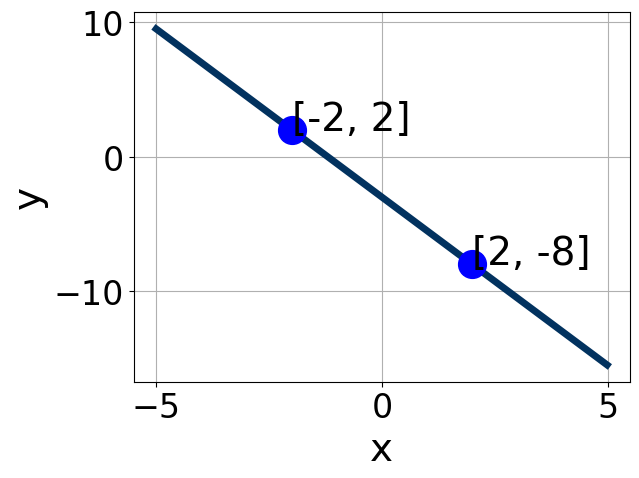
\includegraphics[width=0.5\textwidth]{../Figures/linearGraphToStandardC.png}
\end{center}
\begin{enumerate}[label=\Alph*.]
\item \( A \in [-1.3, 1.7], \hspace{3mm} B \in [0.2, 3.1], \text{ and } \hspace{3mm} C \in [1, 8] \)
\item \( A \in [-1.3, 1.7], \hspace{3mm} B \in [-1.1, -0.2], \text{ and } \hspace{3mm} C \in [-4, 0] \)
\item \( A \in [2.1, 4.2], \hspace{3mm} B \in [-7.5, -4.9], \text{ and } \hspace{3mm} C \in [-12, -8] \)
\item \( A \in [-7.1, -1.5], \hspace{3mm} B \in [-7.5, -4.9], \text{ and } \hspace{3mm} C \in [-12, -8] \)
\item \( A \in [2.1, 4.2], \hspace{3mm} B \in [3.5, 6.6], \text{ and } \hspace{3mm} C \in [9, 12] \)

\end{enumerate} }
\litem{
Solve the equation below. Then, choose the interval that contains the solution.\[ -10(-14x -2) = -19(15x + 12) \]\begin{enumerate}[label=\Alph*.]
\item \( x \in [0.48, 0.6] \)
\item \( x \in [-0.59, -0.54] \)
\item \( x \in [-0.51, -0.44] \)
\item \( x \in [-1.55, -1.31] \)
\item \( \text{There are no real solutions.} \)

\end{enumerate} }
\litem{
Solve the linear equation below. Then, choose the interval that contains the solution.\[ \frac{-5x + 8}{7} - \frac{3x + 4}{5} = \frac{-7x -8}{6} \]\begin{enumerate}[label=\Alph*.]
\item \( x \in [10.35, 14.35] \)
\item \( x \in [81.29, 83.29] \)
\item \( x \in [-1.32, 4.68] \)
\item \( x \in [21.19, 27.19] \)
\item \( \text{There are no real solutions.} \)

\end{enumerate} }
\litem{
Find the equation of the line described below. Write the linear equation as $ y=mx+b $ and choose the intervals that contain $m$ and $b$.\[ \text{Parallel to } 4 x + 7 y = 8 \text{ and passing through the point } (-4, -5). \]\begin{enumerate}[label=\Alph*.]
\item \( m \in [-1.01, 0.15] \hspace*{3mm} b \in [-2.5, 0.1] \)
\item \( m \in [-1.01, 0.15] \hspace*{3mm} b \in [7, 7.4] \)
\item \( m \in [-1.89, -0.59] \hspace*{3mm} b \in [-8.5, -4.9] \)
\item \( m \in [0.51, 1.79] \hspace*{3mm} b \in [-3.2, -1.8] \)
\item \( m \in [-1.01, 0.15] \hspace*{3mm} b \in [-8.5, -4.9] \)

\end{enumerate} }
\litem{
First, find the equation of the line containing the two points below. Then, write the equation as $ y=mx+b $ and choose the intervals that contain $m$ and $b$.\[ (-7, 9) \text{ and } (-2, 7) \]\begin{enumerate}[label=\Alph*.]
\item \( m \in [-1.8, -0.22] \hspace*{3mm} b \in [-6.28, -6.09] \)
\item \( m \in [-1.8, -0.22] \hspace*{3mm} b \in [8.45, 10.98] \)
\item \( m \in [-1.8, -0.22] \hspace*{3mm} b \in [6.1, 6.76] \)
\item \( m \in [-1.8, -0.22] \hspace*{3mm} b \in [15.07, 16.95] \)
\item \( m \in [-0.19, 0.69] \hspace*{3mm} b \in [6.87, 8.48] \)

\end{enumerate} }
\litem{
Solve the linear equation below. Then, choose the interval that contains the solution.\[ \frac{-3x + 3}{2} - \frac{-7x + 8}{6} = \frac{-5x + 5}{4} \]\begin{enumerate}[label=\Alph*.]
\item \( x \in [-2.94, -1.05] \)
\item \( x \in [-0.57, 1.05] \)
\item \( x \in [10.05, 10.98] \)
\item \( x \in [0.99, 1.37] \)
\item \( \text{There are no real solutions.} \)

\end{enumerate} }
\litem{
Find the equation of the line described below. Write the linear equation as $ y=mx+b $ and choose the intervals that contain $m$ and $b$.\[ \text{Parallel to } 5 x - 9 y = 4 \text{ and passing through the point } (-4, 5). \]\begin{enumerate}[label=\Alph*.]
\item \( m \in [-0.52, 1.08] \hspace*{3mm} b \in [-9.22, -5.22] \)
\item \( m \in [1.23, 3] \hspace*{3mm} b \in [6.22, 8.22] \)
\item \( m \in [-0.52, 1.08] \hspace*{3mm} b \in [6.22, 8.22] \)
\item \( m \in [-1.4, 0.4] \hspace*{3mm} b \in [-1.22, 5.78] \)
\item \( m \in [-0.52, 1.08] \hspace*{3mm} b \in [9, 13] \)

\end{enumerate} }
\litem{
Solve the equation below. Then, choose the interval that contains the solution.\[ -5(14x + 19) = -9(12x + 6) \]\begin{enumerate}[label=\Alph*.]
\item \( x \in [-2.5, 0.8] \)
\item \( x \in [-0.1, 1.4] \)
\item \( x \in [3.7, 5.2] \)
\item \( x \in [-4.3, -3.8] \)
\item \( \text{There are no real solutions.} \)

\end{enumerate} }
\litem{
First, find the equation of the line containing the two points below. Then, write the equation as $ y=mx+b $ and choose the intervals that contain $m$ and $b$.\[ (10, -9) \text{ and } (9, -5) \]\begin{enumerate}[label=\Alph*.]
\item \( m \in [-4, -3] \hspace*{3mm} b \in [-31, -25] \)
\item \( m \in [-4, -3] \hspace*{3mm} b \in [-15, -9] \)
\item \( m \in [-4, -3] \hspace*{3mm} b \in [-22, -17] \)
\item \( m \in [-4, -3] \hspace*{3mm} b \in [26, 36] \)
\item \( m \in [2, 5] \hspace*{3mm} b \in [-44, -39] \)

\end{enumerate} }
\litem{
Write the equation of the line in the graph below in Standard form $Ax+By=C$. Then, choose the intervals that contain $A, B, \text{ and } C$.
\begin{center}
    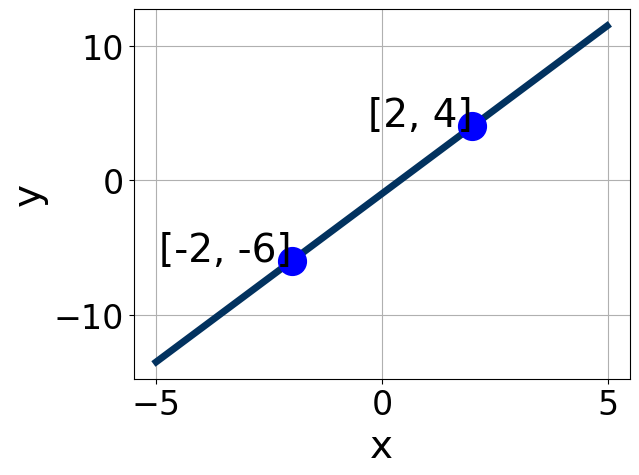
\includegraphics[width=0.5\textwidth]{../Figures/linearGraphToStandardCopyC.png}
\end{center}
\begin{enumerate}[label=\Alph*.]
\item \( A \in [0.2, 2.2], \hspace{3mm} B \in [-1.27, 0.39], \text{ and } \hspace{3mm} C \in [-2.27, -0.83] \)
\item \( A \in [3.9, 8.7], \hspace{3mm} B \in [3.97, 5.85], \text{ and } \hspace{3mm} C \in [3.12, 5.47] \)
\item \( A \in [0.2, 2.2], \hspace{3mm} B \in [-0.05, 2.33], \text{ and } \hspace{3mm} C \in [-0.55, 1.05] \)
\item \( A \in [3.9, 8.7], \hspace{3mm} B \in [-4.23, -3.27], \text{ and } \hspace{3mm} C \in [-4.44, -3.8] \)
\item \( A \in [-8.2, -3.5], \hspace{3mm} B \in [-4.23, -3.27], \text{ and } \hspace{3mm} C \in [-4.44, -3.8] \)

\end{enumerate} }
\end{enumerate}

\end{document}